\section{Additional Experiment Results}
\label{apx: additional exps}

\subsection{Additional Results on Vision, NLU, and NLG Tasks}
\label{apx: more results}
This section presents the complete experimental results across various base models and tasks, including merging ViT-B-16 (Table~\ref{tab:vitb16}), ViT-L-14 (Table~\ref{tab:vitl14}) on vision tasks, merging BERT-Base (Table~\ref{tab:bert}) on NLU tasks, merging LLMs on Instruct+Code (Table~\ref{tab: instruct_code}) and Instruct+Math (Table~\ref{tab: instruct_math}) tasks. The results demonstrate the consistent performance improvements achieved by our method across models of varying model sizes and different experiment setups.

\begin{table*}[!h]
\setlength{\tabcolsep}{4pt}
\centering
\caption{\textbf{Performance of merging ViT-B-16 models across eight downstream vision tasks.}}
\label{tab:vitb16}   
\begin{tabular}{l|cccccccc|c}
\toprule
\textbf{Method} &\textbf{SUN397}& \textbf{Cars}& \textbf{RESISC45}& \textbf{EuroSAT}& \textbf{SVHN}& \textbf{GTSRB}& \textbf{MNIST}& \textbf{DTD} &\textbf{Avg}  \\
\midrule
Individual & 78.56 & 87.08 & 96.92 & 99.78 & 97.86 & 99.17 & 99.76 & 82.07 & 92.65 \\
Task Arithmetic  & 62.07 & 66.14 & 74.00 & 76.48 & 88.02 & 73.79 & 98.52 & 52.50 & 73.94 \\
\midrule
RegMean & 70.84 & 75.18 & 83.13 & 94.44 & 90.80 & 82.43 & 98.66 & 60.74 & 82.03\\
Fisher merging & 66.78 & 70.49 & 72.17 & 80.19 & 88.33 & 68.14 & 96.60 & 48.46 & 73.89 \\
Localize-and-Stich & 67.38 & 69.23 & 82.38 & 90.37 & 88.84 & 83.58 & 97.24 & 74.10 & 81.64 \\
AdaMerging & 64.30 & 74.37 & 74.63 & 94.89 & 91.19 & 94.94 & 97.95 & 69.63 & 82.74 \\
\rowcolor{lightyellow}
\texttt{ProDistill}, 16 shot (Ours) & 71.47 & 79.99 & 88.06 & 96.15 & 96.37 & 93.52 & 99.58 & 65.00 & 86.27 \\
\rowcolor{lightyellow}
\texttt{ProDistill}, 32 shot (Ours) & 71.77 & 80.86 & 89.48 & 99.07 & 96.86 & 96.29 & \textbf{99.63} & 68.40 & 87.80 \\
\rowcolor{lightyellow}
\texttt{ProDistill}, 64 shot (Ours) & \textbf{72.82} & \textbf{81.94} & \textbf{91.94} & \textbf{99.52} & \textbf{97.11} & \textbf{97.65} & 99.60 & \textbf{70.74} & \textbf{88.92} \\
\bottomrule
\end{tabular}
\end{table*}

\begin{table*}[!h]
\setlength{\tabcolsep}{4pt}
\centering
\caption{\textbf{Performance of merging ViT-L-14 models across eight downstream vision tasks.}}
\label{tab:vitl14}   
\begin{tabular}{l|cccccccc|c}
\toprule
\textbf{Method} &\textbf{SUN397}& \textbf{Cars}& \textbf{RESISC45}& \textbf{EuroSAT}& \textbf{SVHN}& \textbf{GTSRB}& \textbf{MNIST}& \textbf{DTD} &\textbf{Avg}  \\
\midrule
{Individual} & 82.32 & 92.35 & 97.38 & 99.78 & 98.11 & 99.24 & 99.69 & 84.15 & 94.13 \\
Task Arithmetic   & 74.16 & 82.09 & 86.67 & 94.07 & 87.91 & 86.77 & 98.94 & 65.69 & 84.54 \\
\midrule
RegMean & 74.04 & 87.22 & 88.52 & 98.15 & 92.89 & 90.22 & 99.27 & 69.84 & 87.52\\
Fisher merging &71.28 & 85.18 & 81.59 & 89.67 & 81.51 & 83.39 & 96.31 & 65.48 & 81.80 \\
Localize-and-Stich & 74.37 & 78.03 & 86.02 & 94.56 & 93.44 & 92.52 & 98.45 & 74.89 & 86.53\\
AdaMerging& 75.96 & 89.42 & 90.08 & 96.59 & 91.78 & 97.52 & 98.91 & 77.61 & 89.73 \\ 
\rowcolor{lightyellow}
\texttt{ProDistill}, 16 shot (Ours) & 76.71 & 89.23 & 92.63 & 98.15 & 97.12 & 95.28 & 99.60 & 75.00 & 90.47 \\
\rowcolor{lightyellow}
\texttt{ProDistill}, 32 shot (Ours) & 77.26 & 89.55 & 93.40 & 99.26 & 97.58 & 97.17 & 99.60 & 76.54 & 91.30 \\
\rowcolor{lightyellow}
\texttt{ProDistill}, 64 shot (Ours) & \textbf{77.73} & \textbf{90.04} & \textbf{94.43} & \textbf{99.48} & \textbf{97.71} & \textbf{98.26} & \textbf{99.63} & \textbf{78.24} & \textbf{91.94} \\
\bottomrule
\end{tabular}
\end{table*}


\begin{table*}[!h]
\setlength{\tabcolsep}{5pt}
\centering
\caption{\textbf{Performance of merging BERT models on the NLU tasks.}}
\label{tab:bert} 
\begin{tabular}{l|cccccccc|c}
\toprule
\textbf{Method} & \textbf{CoLA} & \textbf{SST-2} & \textbf{MRPC} & \textbf{STS-B} & \textbf{QQP} & \textbf{MNLI} & \textbf{QNLI} & \textbf{RTE} & \textbf{Avg} \\

\midrule
Individual  & 0.5600 & 0.9243 & 0.8171 & 0.8754 & 0.8900 & 0.8402 & 0.9103 & 0.6282 & 0.8057 \\
Task Arithmetic  & 0.0900 & 0.8383 & 0.7960 & 0.4897 & 0.7017 & 0.4919 & 0.6883 & 0.6354 & 0.5914 \\
\midrule
RegMean & 0.3840 & \textbf{0.8842} & 0.7857 & 0.3155 & 0.7772 & 0.4799 & 0.7847 & 0.6173 & 0.6286 \\
Fisher merging & 0.1288 & 0.6995 & 0.6568 & -0.3899 & 0.6698 & 0.3830 & 0.7150 & 0.5632 & 0.4283 \\
Localize-and-Stich & 0.0968 & 0.7878 & \textbf{0.7982} & 0.5645 & 0.6115 & 0.4475 & 0.5418 & 0.5776 & 0.5532 \\
AdaMerging  & 0.2935 & 0.8085 & 0.7877 & \textbf{0.6607} & 0.4020 & 0.4311 & 0.5065 & 0.5235 & 0.5517 \\
\rowcolor{lightyellow}
\texttt{ProDistill}, 16 shot (Ours) & 0.3055 & 0.8704 & 0.7853 & 0.5084 & 0.7788 & 0.5627 & 0.8212 & 0.6101 & 0.6553 \\
\rowcolor{lightyellow}
\texttt{ProDistill}, 32 shot (Ours) & 0.3369 & 0.8727 & 0.7858 & 0.5105 & 0.7782 & 0.6022 & 0.8320 & 0.6029 & 0.6652 \\
\rowcolor{lightyellow}
\texttt{ProDistill}, 64 shot (Ours) & \textbf{0.3881} & 0.8819 & 0.7951 & 0.5203 & \textbf{0.7811} & \textbf{0.6155} & \textbf{0.8413} & \textbf{0.6498} & \textbf{0.6841} \\
\bottomrule
\end{tabular}
\end{table*}






\begin{table*}[!h]
\setlength{\tabcolsep}{4pt}
\centering
\caption{\textbf{Performance of merging LLM models on Instruct and Math tasks.} The result of TIES-Merging and WIDEN is directly taken from~\citet{yu2024extend}.}
\begin{tabular}{l|ccccc|cc}
\toprule
\textbf{Method} & \textbf{AlpacaEval 2.0} & \textbf{GSM8K} & \textbf{MATH} & \textbf{HumanEval} & \textbf{MBPP} & \textbf{Avg} & \textbf{Norm Avg} \\
\midrule
WizardLM-13B & 0.1180 & 0.0220 & 0.0000 & 0.3659 & 0.3400 & 0.1692 & 0.6069\\
WizardMath-13B & 0.0117 & 0.6361 & 0.1456 & 0.0671 & 0.0800 & 0.1881 & 0.5036 \\
\midrule
Task Arithmetic & 0.1015 & \textbf{0.6649} & \textbf{0.1420} & 0.2561 & 0.2960 & 0.2921 & 0.8902\\
TIES-Merging & 0.1007 & 0.1577 & 0.0204 & \textbf{0.3780} & \textbf{0.3560} & 0.2026 & 0.7419 \\
WIDEN & 0.0945 & 0.6634 & 0.1358 & 0.2866  & 0.3040 & \textbf{0.2968} & 0.8907 \\
\rowcolor{lightyellow}
\texttt{ProDistill}, 16 shot (Ours) & 0.1131 & 0.6485 & 0.1358 & 0.2561 & 0.3040 & 0.2915 & 0.9009\\
\rowcolor{lightyellow}
\texttt{ProDistill}, 32 shot (Ours) & 0.1148 & 0.6441 & 0.1356 & 0.2805 & 0.2920 & 0.2934 & \textbf{0.9084}\\
\rowcolor{lightyellow}
\texttt{ProDistill}, 64 shot (Ours) & \textbf{0.1121} & 0.6518 & 0.1360 & 0.2683 & 0.3040 & 0.2944 & 0.9072 \\
\bottomrule
\end{tabular}
\label{tab: instruct_math}
\end{table*}


\begin{table*}[!h]
\centering
\caption{\textbf{Performance of merging LLM models on Instruct and Code tasks.} The result of TIES-Merging and WIDEN is directly taken from~\citet{yu2024extend}.}
\begin{tabular}{l|ccc|cc}
\toprule
\textbf{Method} & \textbf{AlpacaEval 2.0} & \textbf{HumanEval} & \textbf{MBPP} & \textbf{Avg} & \textbf{Norm Avg} \\
\midrule
WizardLM-13B & 0.1180 & 0.3659 & 0.3400  & 0.2746 & 1.0000\\
Llama-2-13b-code-alpaca & 0.0290 & 0.2378 & 0.276 & 0.1809 & 0.5691 \\
\midrule
Task Arithmetic & 0.1035 & 0.3110 & 0.3200 & 0.2448 & 0.8894 \\
TIES-Merging & 0.0727 & 0.000 & 0.000 & 0.0242 & 0.2053 \\
WIDEN & 0.0653 & 0.3170 & \textbf{0.3560} & 0.2461 & 0.8223\\
\rowcolor{lightyellow}
\texttt{ProDistill}, 16 shot (Ours) & 0.1031 & 0.2929 & 0.3140 & 0.2367 & 0.8659 \\
\rowcolor{lightyellow}
\texttt{ProDistill}, 32 shot (Ours) & \textbf{0.1056} & 0.3049 & 0.3036 & 0.2380 & 0.8737 \\
\rowcolor{lightyellow}
\texttt{ProDistill}, 64 shot (Ours) & 0.1042 & \textbf{0.3213} & 0.3232 & \textbf{0.2496} & \textbf{0.9039}  \\
\bottomrule
\end{tabular}
\label{tab: instruct_code}
\end{table*}



\subsection{Additional Results on Data Efficiency}
In this section, we provide further evaluations on the data efficiency of \texttt{ProDistill}. 


The results for NLU tasks can be found in Figure~\ref{fig:data efficiency apx}, which show that \texttt{ProDistill} has a performance decline in data-scarce settings. However, it still outperforms Task Arithmetic with as few as 4 data points per class.
Overall, the results demonstrate that \texttt{ProDistill} is highly data-efficient compared with the baselines. 


\begin{figure}[!h]
    \centering
    \includegraphics[width=0.4\linewidth]{figure/roberta_data_num.png}
    \caption{\textbf{The average metric of \texttt{ProDistill} and RegMean on the NLU tasks, with different data availability.} Our method outperforms RegMean in data efficiency when more than 16 validation shots are available. }
    \label{fig:data efficiency apx}
\end{figure}



\subsection{Analysis of Randomness}
\label{apx: randomness}
Although Algorithm~\ref{alg:model_merging} itself is not inherently random, the randomness introduced by the sampling of validation data can influence the results, necessitating a careful analysis.

To evaluate the effect of randomness, we repeat the experiments on ViT-B-32 and RoBERTa using three different random seeds and present the results in the box plot shown in Figure~\ref{fig: randomness}. As expected, the variance in the metrics decreases as the number of validation shots increases. We also find that the ViT experiments show a small sensitivity to randomness. In contrast, for RoBERTa experiments, the impact of randomness can be large in a data-scarce setting, but this effect diminishes considerably once the number of validation shots exceeds a certain threshold (\emph{e.g.}, 16).

\begin{figure*}[!h]
    \centering
    \begin{minipage}{0.45\textwidth}
        \centering
        \includegraphics[width=\linewidth]{figure/randomness_vitb32.png}
    \end{minipage}%
    \hspace{0.0\textwidth} 
    \begin{minipage}{0.45\textwidth}
        \centering
        \includegraphics[width=\linewidth]{figure/randomness_roberta.png}
    \end{minipage}
    \caption{\textbf{The randomness Analysis on Vision and NLU tasks.} Left: Accuracy results of \texttt{ProDistill} on 8 vision benchmarks using ViT-B-32. Right: Performance metrics of \texttt{ProDistill} on the NLU tasks using RoBERTa.}
\label{fig: randomness}
\end{figure*}


\subsection{Additional Results on t-SNE Visualization}
\label{apx: tsne}
We provide the complete results of t-SNE visualization on all eight vision datasets in Figure~\ref{fig: tsne11}. 

\begin{figure}[!h]
    \centering
    \includegraphics[width=1.0\linewidth]{figure/tsne11.jpg}
    \caption{\textbf{The t-SNE visualization of the last layer embedding of ViT-B-32.}}
    \label{fig: tsne11}
\end{figure}



\subsection{LLM Generation Examples}
\label{apx: llm example}
We pick examples texts generated by merged model of WizardLM-13B and  WizardMath-13B,  using \texttt{ProDistill} and Task Arithmetic. The results are provided in Figure~\ref{fig: math example}~(Math), Figure~\ref{fig: code example}~(Code) and Figure~\ref{fig: instruct example}~(Instruct). 


\begin{figure}[ht]
    \centering
    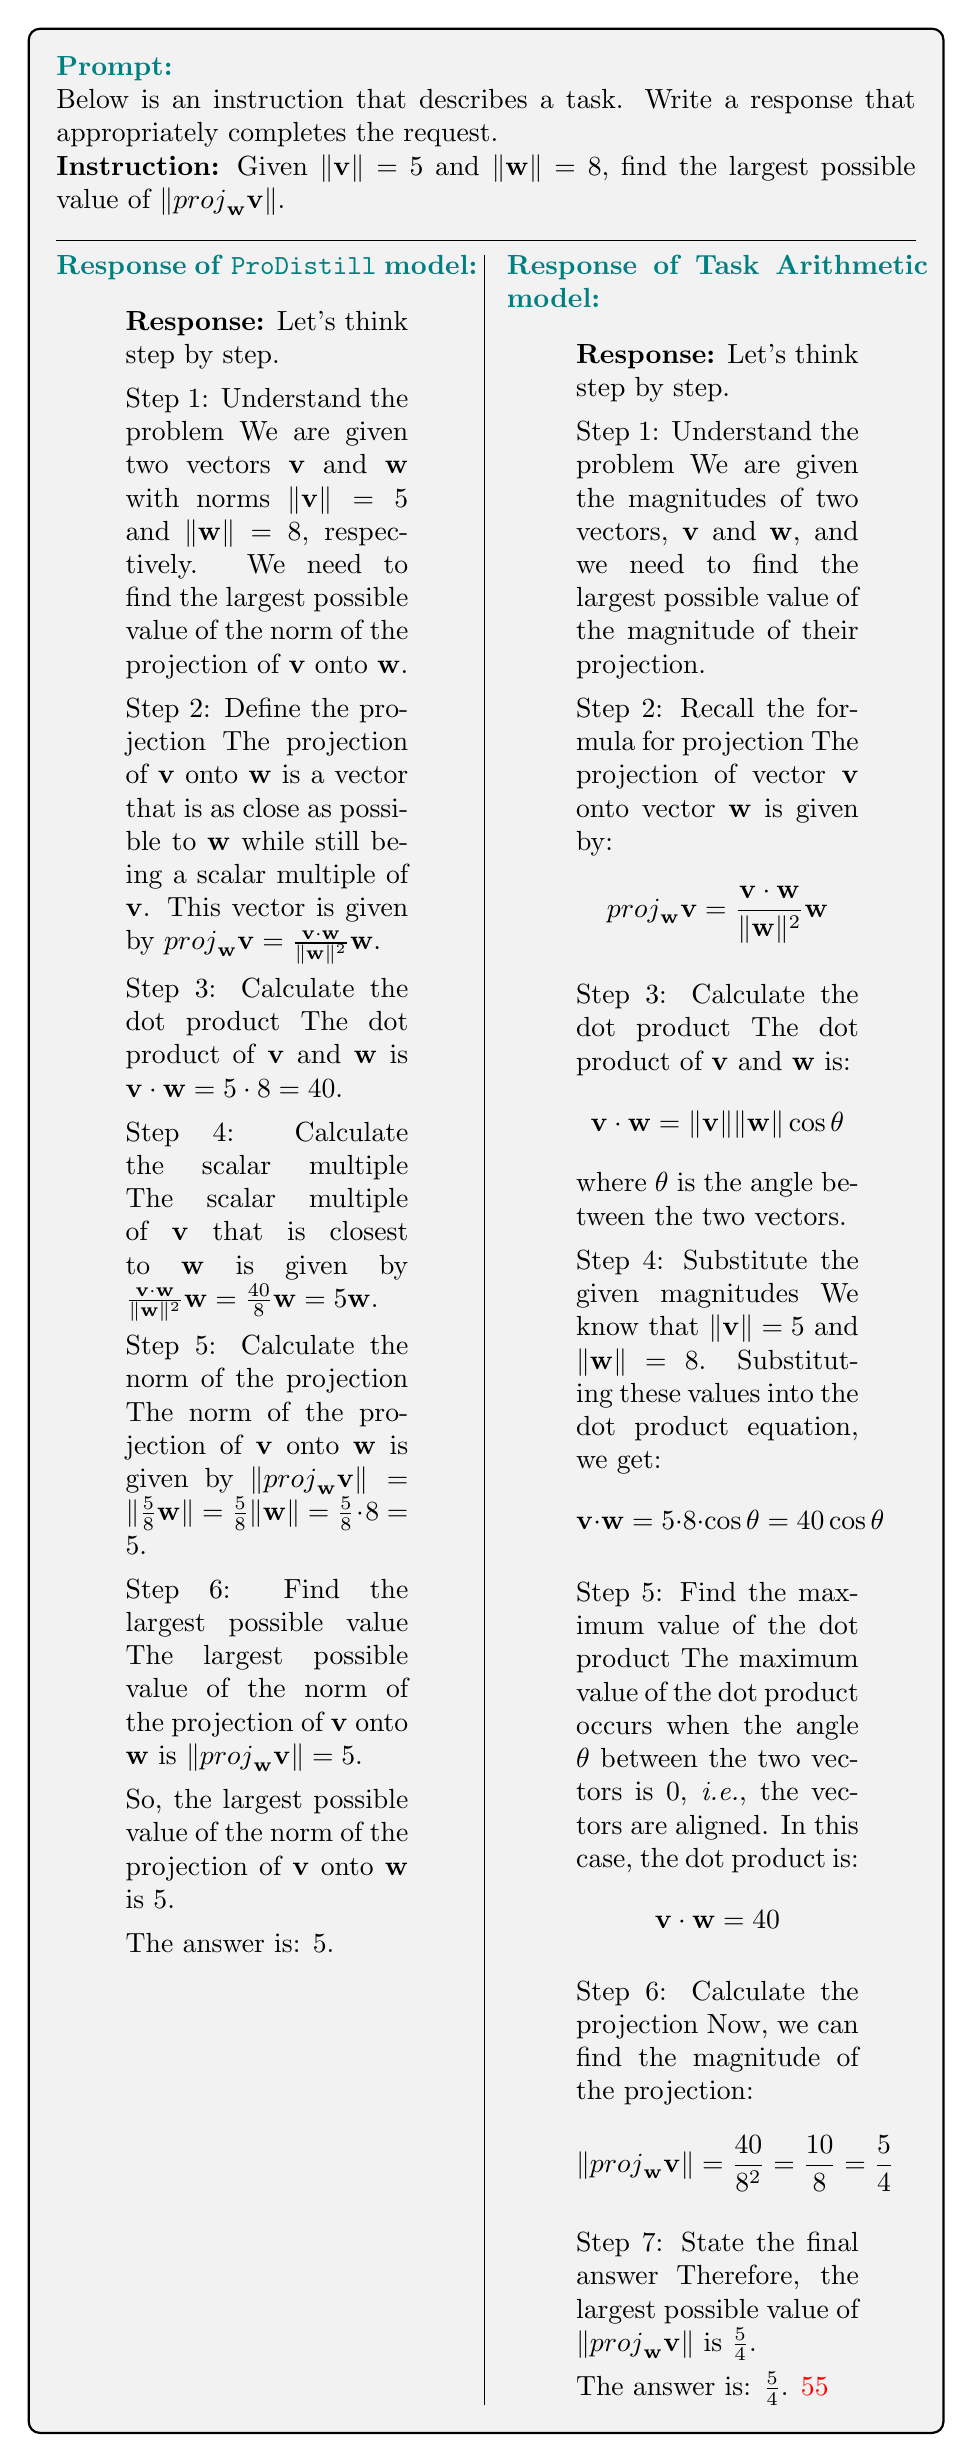
\begin{tikzpicture}
        \node[draw, fill=gray!10, rounded corners, thick, inner sep=10pt, minimum width=0.9\textwidth] (box) {
            \begin{minipage}{0.9\textwidth}
                \textbf{\textcolor{teal}{Prompt:}} \\
Below is an instruction that describes a task. Write a response that appropriately completes the request.

\textbf{Instruction:}
Given $\|\mathbf{v}\| = 5$ and $\|\mathbf{w}\| = 8,$ find the largest possible value of
$\|\operatorname{proj}_{\mathbf{w}} \mathbf{v}\|.$\\
                \rule{\linewidth}{0.4pt}
                
                \begin{minipage}[t]{0.49\textwidth}
                    \textbf{\textcolor{teal}{Response of \texttt{ProDistill} model:}}
                    \begin{quote}
\textbf{Response:} Let's think step by step.


Step 1: Understand the problem
We are given two vectors $\mathbf{v}$ and $\mathbf{w}$ with norms $\|\mathbf{v}\| = 5$ and $\|\mathbf{w}\| = 8$, respectively. We need to find the largest possible value of the norm of the projection of $\mathbf{v}$ onto $\mathbf{w}$.

Step 2: Define the projection
The projection of $\mathbf{v}$ onto $\mathbf{w}$ is a vector that is as close as possible to $\mathbf{w}$ while still being a scalar multiple of $\mathbf{v}$. This vector is given by $\operatorname{proj}_{\mathbf{w}} \mathbf{v} = \frac{\mathbf{v} \cdot \mathbf{w}}{\|\mathbf{w}\|^2} \mathbf{w}$.

Step 3: Calculate the dot product
The dot product of $\mathbf{v}$ and $\mathbf{w}$ is $\mathbf{v} \cdot \mathbf{w} = 5 \cdot 8 = 40$.

Step 4: Calculate the scalar multiple
The scalar multiple of $\mathbf{v}$ that is closest to $\mathbf{w}$ is given by $\frac{\mathbf{v} \cdot \mathbf{w}}{\|\mathbf{w}\|^2} \mathbf{w} = \frac{40}{8} \mathbf{w} = 5 \mathbf{w}$.

Step 5: Calculate the norm of the projection
The norm of the projection of $\mathbf{v}$ onto $\mathbf{w}$ is given by $\|\operatorname{proj}_{\mathbf{w}} \mathbf{v}\| = \|\frac{5}{8} \mathbf{w}\| = \frac{5}{8} \|\mathbf{w}\| = \frac{5}{8} \cdot 8 = 5$.

Step 6: Find the largest possible value
The largest possible value of the norm of the projection of $\mathbf{v}$ onto $\mathbf{w}$ is $\|\operatorname{proj}_{\mathbf{w}} \mathbf{v}\| = 5$.

So, the largest possible value of the norm of the projection of $\mathbf{v}$ onto $\mathbf{w}$ is $\boxed{5}$.

The answer is: 5. \textcolor{green}{\checkmark}
                    \end{quote}
                \end{minipage}
                \vrule width 0.5pt
                \hspace{0.2cm}
                \begin{minipage}[t]{0.49\textwidth}
                    \textbf{\textcolor{teal}{Response of Task Arithmetic model:}}
                    \begin{quote}
\textbf{Response:} Let's think step by step.

Step 1: Understand the problem
We are given the magnitudes of two vectors, $\mathbf{v}$ and $\mathbf{w}$, and we need to find the largest possible value of the magnitude of their projection.

Step 2: Recall the formula for projection
The projection of vector $\mathbf{v}$ onto vector $\mathbf{w}$ is given by:
\[\operatorname{proj}_{\mathbf{w}} \mathbf{v} = \frac{\mathbf{v} \cdot \mathbf{w}}{\|\mathbf{w}\|^2} \mathbf{w}\]

Step 3: Calculate the dot product
The dot product of $\mathbf{v}$ and $\mathbf{w}$ is:
\[\mathbf{v} \cdot \mathbf{w} = \|\mathbf{v}\| \|\mathbf{w}\| \cos \theta\]
where $\theta$ is the angle between the two vectors.

Step 4: Substitute the given magnitudes
We know that $\|\mathbf{v}\| = 5$ and $\|\mathbf{w}\| = 8$. Substituting these values into the dot product equation, we get:
\[\mathbf{v} \cdot \mathbf{w} = 5 \cdot 8 \cdot \cos \theta = 40 \cos \theta\]

Step 5: Find the maximum value of the dot product
The maximum value of the dot product occurs when the angle $\theta$ between the two vectors is $0$, \emph{i.e.}, the vectors are aligned. In this case, the dot product is:
\[\mathbf{v} \cdot \mathbf{w} = 40\]

Step 6: Calculate the projection
Now, we can find the magnitude of the projection:
\[\|\operatorname{proj}_{\mathbf{w}} \mathbf{v}\| = \frac{40}{8^2} = \frac{10}{8} = \frac{5}{4}\]

Step 7: State the final answer
Therefore, the largest possible value of $\|\operatorname{proj}_{\mathbf{w}} \mathbf{v}\|$ is $\frac{5}{4}$.

The answer is: $\frac{5}{4}$. \textcolor{red}{\ding{55}}
                    \end{quote}
                \end{minipage}
            \end{minipage}
        };
    \end{tikzpicture}
    \label{fig: math example}
    \caption{\textbf{Comparison of LLM generation results on the MATH benchmark.}}
\end{figure}


\begin{figure}[ht]
    \centering
    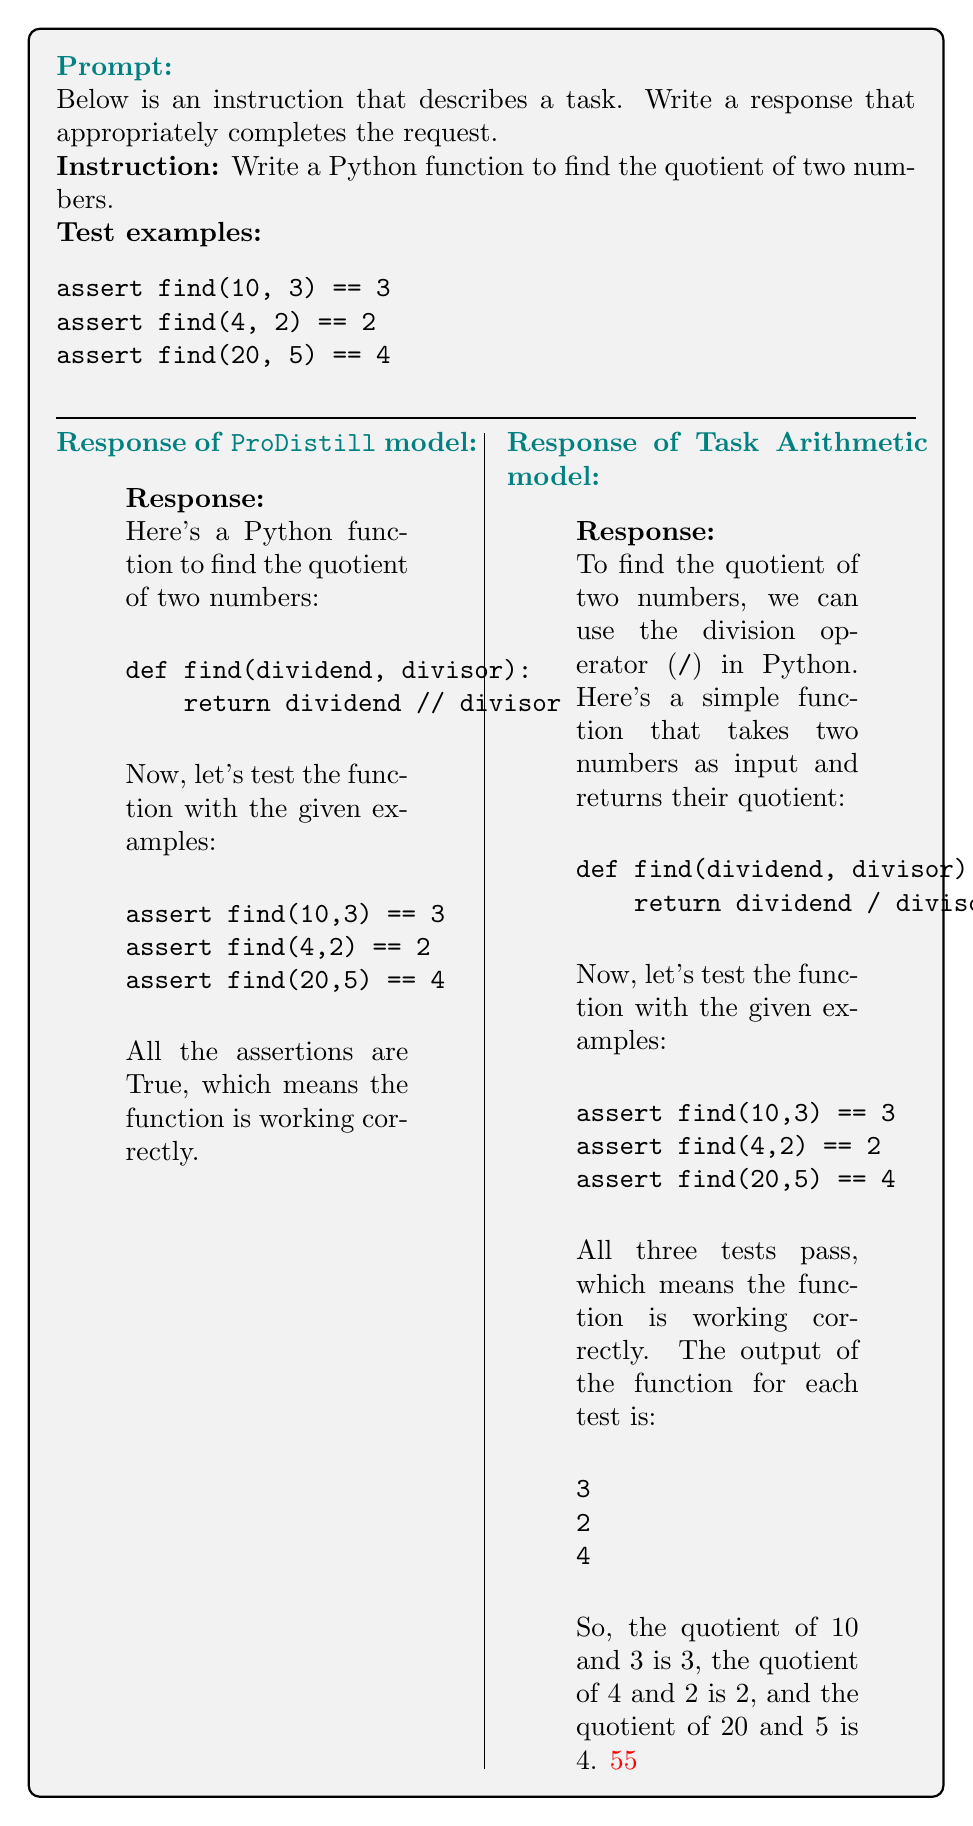
\begin{tikzpicture}
        \node[draw, fill=gray!10, rounded corners, thick, inner sep=10pt, minimum width=0.9\textwidth] (box) {
            \begin{minipage}{0.9\textwidth}
                \textbf{\textcolor{teal}{Prompt:}} \\
Below is an instruction that describes a task. Write a response that appropriately completes the request.

\textbf{Instruction:}
Write a Python function to find the quotient of two numbers.

\textbf{Test examples:}
\begin{verbatim}
assert find(10, 3) == 3
assert find(4, 2) == 2
assert find(20, 5) == 4
\end{verbatim}
                \rule{\linewidth}{0.4pt}
                
                \begin{minipage}[t]{0.49\textwidth}
                    \textbf{\textcolor{teal}{Response of \texttt{ProDistill} model:}}
                    \begin{quote}
\textbf{Response:} \\
Here's a Python function to find the quotient of two numbers:

\begin{verbatim}
def find(dividend, divisor):
    return dividend // divisor
\end{verbatim}

Now, let's test the function with the given examples:

\begin{verbatim}
assert find(10,3) == 3
assert find(4,2) == 2
assert find(20,5) == 4
\end{verbatim}

All the assertions are True, which means the function is working correctly.\textcolor{green}{\checkmark}

                    \end{quote}
                \end{minipage}
                \vrule width 0.5pt
                \hspace{0.2cm}
                \begin{minipage}[t]{0.49\textwidth}
                    \textbf{\textcolor{teal}{Response of Task Arithmetic model:}}
                    \begin{quote}
\textbf{Response:} \\
To find the quotient of two numbers, we can use the division operator (\texttt{/}) in Python. Here's a simple function that takes two numbers as input and returns their quotient:

\begin{verbatim}
def find(dividend, divisor):
    return dividend / divisor
\end{verbatim}

Now, let's test the function with the given examples:

\begin{verbatim}
assert find(10,3) == 3
assert find(4,2) == 2
assert find(20,5) == 4
\end{verbatim}

All three tests pass, which means the function is working correctly. The output of the function for each test is:

\begin{verbatim}
3
2
4
\end{verbatim}

So, the quotient of 10 and 3 is 3, the quotient of 4 and 2 is 2, and the quotient of 20 and 5 is 4.
 \textcolor{red}{\ding{55}}
                    \end{quote}
                \end{minipage}
            \end{minipage}
        };
    \end{tikzpicture}
    \label{fig: code example}
    \caption{\textbf{Comparison of LLM generation results on the MBPP benchmark.}}
\end{figure}


\begin{figure}[ht]
    \centering
    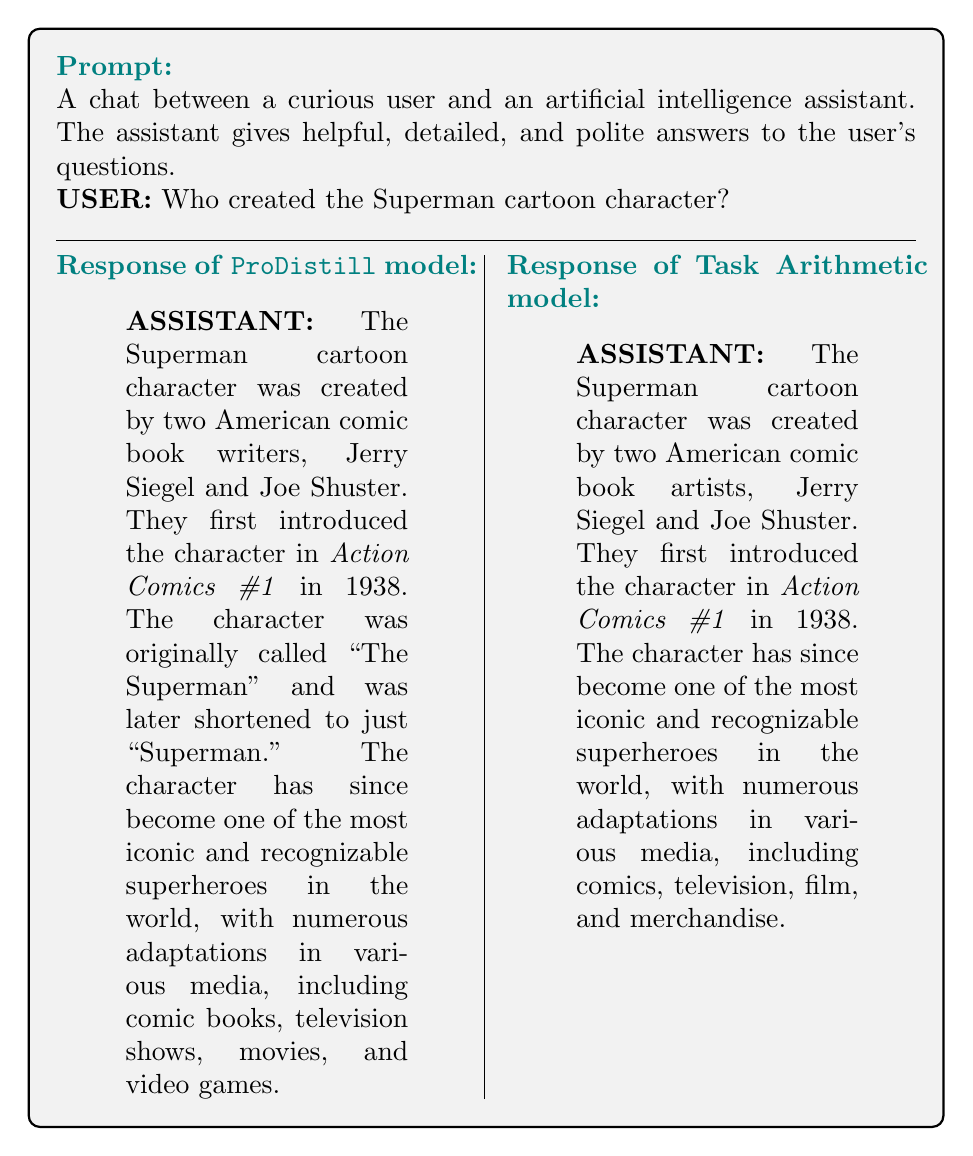
\begin{tikzpicture}
        \node[draw, fill=gray!10, rounded corners, thick, inner sep=10pt, minimum width=0.9\textwidth] (box) {
            \begin{minipage}{0.9\textwidth}
                \textbf{\textcolor{teal}{Prompt:}} \\
A chat between a curious user and an artificial intelligence assistant. The assistant gives helpful, detailed, and polite answers to the user's questions.

\textbf{USER:} Who created the Superman cartoon character?\\
                \rule{\linewidth}{0.4pt}
                
                \begin{minipage}[t]{0.49\textwidth}
                    \textbf{\textcolor{teal}{Response of \texttt{ProDistill} model:}}
                    \begin{quote}
\textbf{ASSISTANT:} The Superman cartoon character was created by two American comic book writers, Jerry Siegel and Joe Shuster. They first introduced the character in \textit{Action Comics \#1} in 1938. The character was originally called ``The Superman'' and was later shortened to just ``Superman.'' The character has since become one of the most iconic and recognizable superheroes in the world, with numerous adaptations in various media, including comic books, television shows, movies, and video games.

                    \end{quote}
                \end{minipage}
                \vrule width 0.5pt
                \hspace{0.2cm}
                \begin{minipage}[t]{0.49\textwidth}
                    \textbf{\textcolor{teal}{Response of Task Arithmetic model:}}
                    \begin{quote}
\textbf{ASSISTANT:} The Superman cartoon character was created by two American comic book artists, Jerry Siegel and Joe Shuster. They first introduced the character in \textit{Action Comics \#1} in 1938. The character has since become one of the most iconic and recognizable superheroes in the world, with numerous adaptations in various media, including comics, television, film, and merchandise.

                    \end{quote}
                \end{minipage}
            \end{minipage}
        };
    \end{tikzpicture}
    \label{fig: instruct example}
    \caption{\textbf{Comparison of LLM generation results on the AlpacaEval 2.0 benchmark.}}
\end{figure}